\pdfoutput=1
\documentclass[a4paper,12pt,titlepage, twoside]{article}
\usepackage[english]{babel}
\usepackage[utf8]{inputenc}
\usepackage{amssymb,amsmath}
\usepackage{algorithm,algpseudocode}
\usepackage[title,titletoc]{appendix}
\newcommand{\Author}{Jan Bouček}
\newcommand{\Title}{Model Predictive Control of Unmanned Helicopter with Obstacle Avoidance}
\newcommand{\Acronym}{Acronym}
\newcommand{\WorkPackage}{WorkPackage}
\newcommand{\DocName}{Bachelor thesis}
\newcommand{\Subject}{\WorkPackage - \DocName}
\newcommand{\Keywords}{mobile robotics}
\newcommand{\Date}{18/05/2016}
\newcommand{\DOCVersion}{0.1}
\newcommand{\jed}[1]{\ensuremath{~\mathrm{#1}}} %příkaz pro sazbu fyzikálních jednotek

\newcommand{\Lagr}{\mathcal{L}}
\newcommand{\uvec}{\textbf{\underline{u}}}
\newcommand{\macJ}{\mathrm{J}(\uvec)}
\newcommand{\urvec}{\textbf{\underline{u}}_r}
\newcommand{\macf}{f(\uvec)}
\newcommand{\macg}{g(\uvec)}
\newcommand{\macoi}{\vec{\omega}_i}
\newcommand{\macU}{\textbf{U}}
\newcommand{\macAr}{\textbf{\^A}}
\newcommand{\macBr}{\textbf{\^B}}
\newcommand{\macHr}{\textbf{\^H}}
\newcommand{\maccr}{\textbf{\^c}}

\def\clinks{false}

\usepackage{graphicx}       %%% graphics for dvips
\usepackage{latexsym}
\usepackage{a4wide}
\usepackage{color} 
\usepackage{indentfirst}
\usepackage{fancyhdr}
\usepackage{longtable}
\usepackage{pifont}
\usepackage{makeidx}
\usepackage{lastpage}
\usepackage{multirow}
\usepackage{dcolumn} 
\usepackage{epstopdf}
\usepackage{url}
\usepackage{listings}
\usepackage{caption}
\usepackage{subcaption}
\usepackage{relsize}
\usepackage{pdfpages}
\usepackage{natbib}
\usepackage{url}
\usepackage{amsmath}
\captionsetup{compatibility=false}
\usepackage{grffile}
\usepackage{tikz}
\usepackage{pgf}
\usepackage{amsmath} 
\usepackage[utf8]{inputenc}
\usepackage{verbatim}
\usetikzlibrary{arrows,automata,shapes,arrows, positioning, calc}


\lstset{breaklines=true,captionpos=b,frame=single,language=sh,float=h}
\lstloadlanguages{sh,c}
\def\lstlistingname{Listing}%{Výpis}
\def\lstlistlistingname{Listings}%{Seznam výpisů}

% European layout (no extra space after `.')
\frenchspacing

% no indent, free space between paragraphs
\setlength{\parindent}{1cm}
\setlength{\parskip}{1ex plus 0.5ex minus 0.2ex}

\usepackage{ifthen} %%% package for conditionals in TeX
\newread\testin
\def\softinput #1 {\let\next=\relax \openin\testin=#1
\ifeof\testin \message{Info: the file #1 does not exist}%
\else \closein\testin \def\next{\input #1 }\fi
\next}

\softinput{makeconfig}

\ifx\clinks\undefined
\def\clinks{true}
\fi

\ifx\pdfoutput\undefined %%% LATEX %%%
\def\nothtml{}  %%% \nothtml is defined if not processed with latex2html
%\usepackage[dvips]{graphicx}       %%% graphics for dvips
\usepackage[                %%% hyper-references for ps2pdf
bookmarks=true,%                   %%% generate bookmarks ...
breaklinks=true,%                  %%% breaks lines, but links are very small
hypertexnames=false,%              %%% needed for correct links to figures
colorlinks=\clinks,%
urlcolor=blue
]{hyperref}           %%% blue instead of cyan URLS
\hypersetup{
pdfcreator  = {LaTeX with hyperref package},
pdfproducer = {dvips + ps2pdf},
}
\else %%% PDFLATEX %%%
\def\nothtml{}  %%% \nothtml is defined if not processed with latex2html
%\usepackage[pdftex]{graphicx}        %%% graphics for pdfLaTeX
\usepackage[              %%% hyper-references for pdflatex
bookmarks=true,%                   %%% generate bookmarks ...
hypertexnames=false,%              %%% needed for correct links to figures
breaklinks=true,%                  %%% break links if exceeding a single line
colorlinks={\clinks},%
urlcolor=blue]{hyperref}           %%% blue instead of cyan URLS
\pdfadjustspacing=1                %%% force LaTeX-like character spacing
\fi

\hypersetup{  
pdfauthor={\Author},
pdftitle={\Title - \Acronym},
pdfsubject={\Subject},
pdfkeywords={\Keywords}
}

\def\BackgroundEPS#1#2#3#4{%
\special{ps: @beginspecial @setspecial initmatrix
0.1 setgray #2 #3 translate #4 dup scale}
\special{ps: plotfile #1}
\special{ps: @endspecial}
}

\pagestyle{fancy}
\setlength{\headheight}{18pt}
\renewcommand{\footrulewidth}{0.4pt}

%\lfoot{ČVUT FEL, Katedra Kybernetiky, Gerstner Laboratory}
\cfoot{}
%\rfoot{\thepage$/$\pageref{LastPage}}

\fancypagestyle{plain}

\fancyhead[R]{}

\newcommand{\DocBegin}{
\ifx\glreport\undefined
\else
\input{../common/glreport}
\fi
}



\tikzset{
    state/.style={
           rectangle,
           draw=black, very thick,
           minimum height=2em,
           text centered,
           },
    input/.style={
           circle,
           draw=black, very thick,
           minimum height=1em,
           text centered,
           },
    nothing/.style={
           rectangle,
           rounded corners,
           draw=white, very thick,
           minimum height=2em,
           inner sep=2pt,
           text centered,
           },
}






\renewcommand{\lstlistlistingname}{List of Algorithms}
\renewcommand{\lstlistingname}{Listing}
\definecolor{background_color}{rgb}{1.0, 1.0, 0.85}
\definecolor{comment_color}{rgb}{0.0, 0.5, 0.0}
\definecolor{keyword_color}{rgb}{0.0, 0.0, 1.0}
\definecolor{string_color}{rgb}{0.8, 0.0, 0.0}
\lstset{language=ksh}
\lstset{backgroundcolor=\color{background_color}}
\lstset{frameround=tttt}
\lstset{columns=fullflexible}
\lstset{keywordstyle=\color{keyword_color}\bfseries}
\lstset{commentstyle=\color{comment_color}}
\lstset{stringstyle=\color{string_color}}
\lstset{basicstyle=\ttfamily}
\lstset{showstringspaces=false}
\lstset{frame=single}
\lstset{keepspaces=true}
\lstset{tabsize=4}
\lstset{breaklines=true}
\lstset{captionpos=b}

\begin{document}
\DocBegin

%% PRINT
%% \setlength{\oddsidemargin}{+0.5cm} 
%% \setlength{\evensidemargin}{-0.5cm}
%%

% Titulní stránka
\begin{titlepage}
\begin{center}

{\Large CZECH TECHNICAL UNIVERSITY IN PRAGUE}
\vskip 10pt

\vskip 8pt
{\Large Faculty of Electrical Engineering}
 
%\vskip 0pt plus 2fill
\vspace{50pt}
{\Huge\bf MASTER'S THESIS}\\
\vspace{40pt}

\includegraphics[width=10cm]{src/lev.pdf}

\vspace{40pt}
{\Large\rm \Author } \\
\vspace{20pt}
{\Large\bf \Title}

\vspace{60pt}
{\bf Department of Cybernetics}\\
\vspace{5pt}
{Thesis supervisor: {\bf Ing. Michal Reinštein, Ph.D.}}

\vspace{30pt}
%{\sc Prague 2013}
\end{center}
\end{titlepage}

\pagestyle{empty}
\cleardoublepage

%% EBOOK
~\vfill{}

\section*{Author statement for undergraduate thesis:}
I declare that the presented work was developed independently and I have listed all sources of information used within in the accordance with the methodical instructions for observing the ethical principles in the preparation of university thesis.

\vspace{1.5cm}
~\\

Prague, date.............................\hfill{}...............................................

\hfill{}~~~~~~~~~~~~~~~

\newpage{}

\cleardoublepage
%%


%% EBOOK
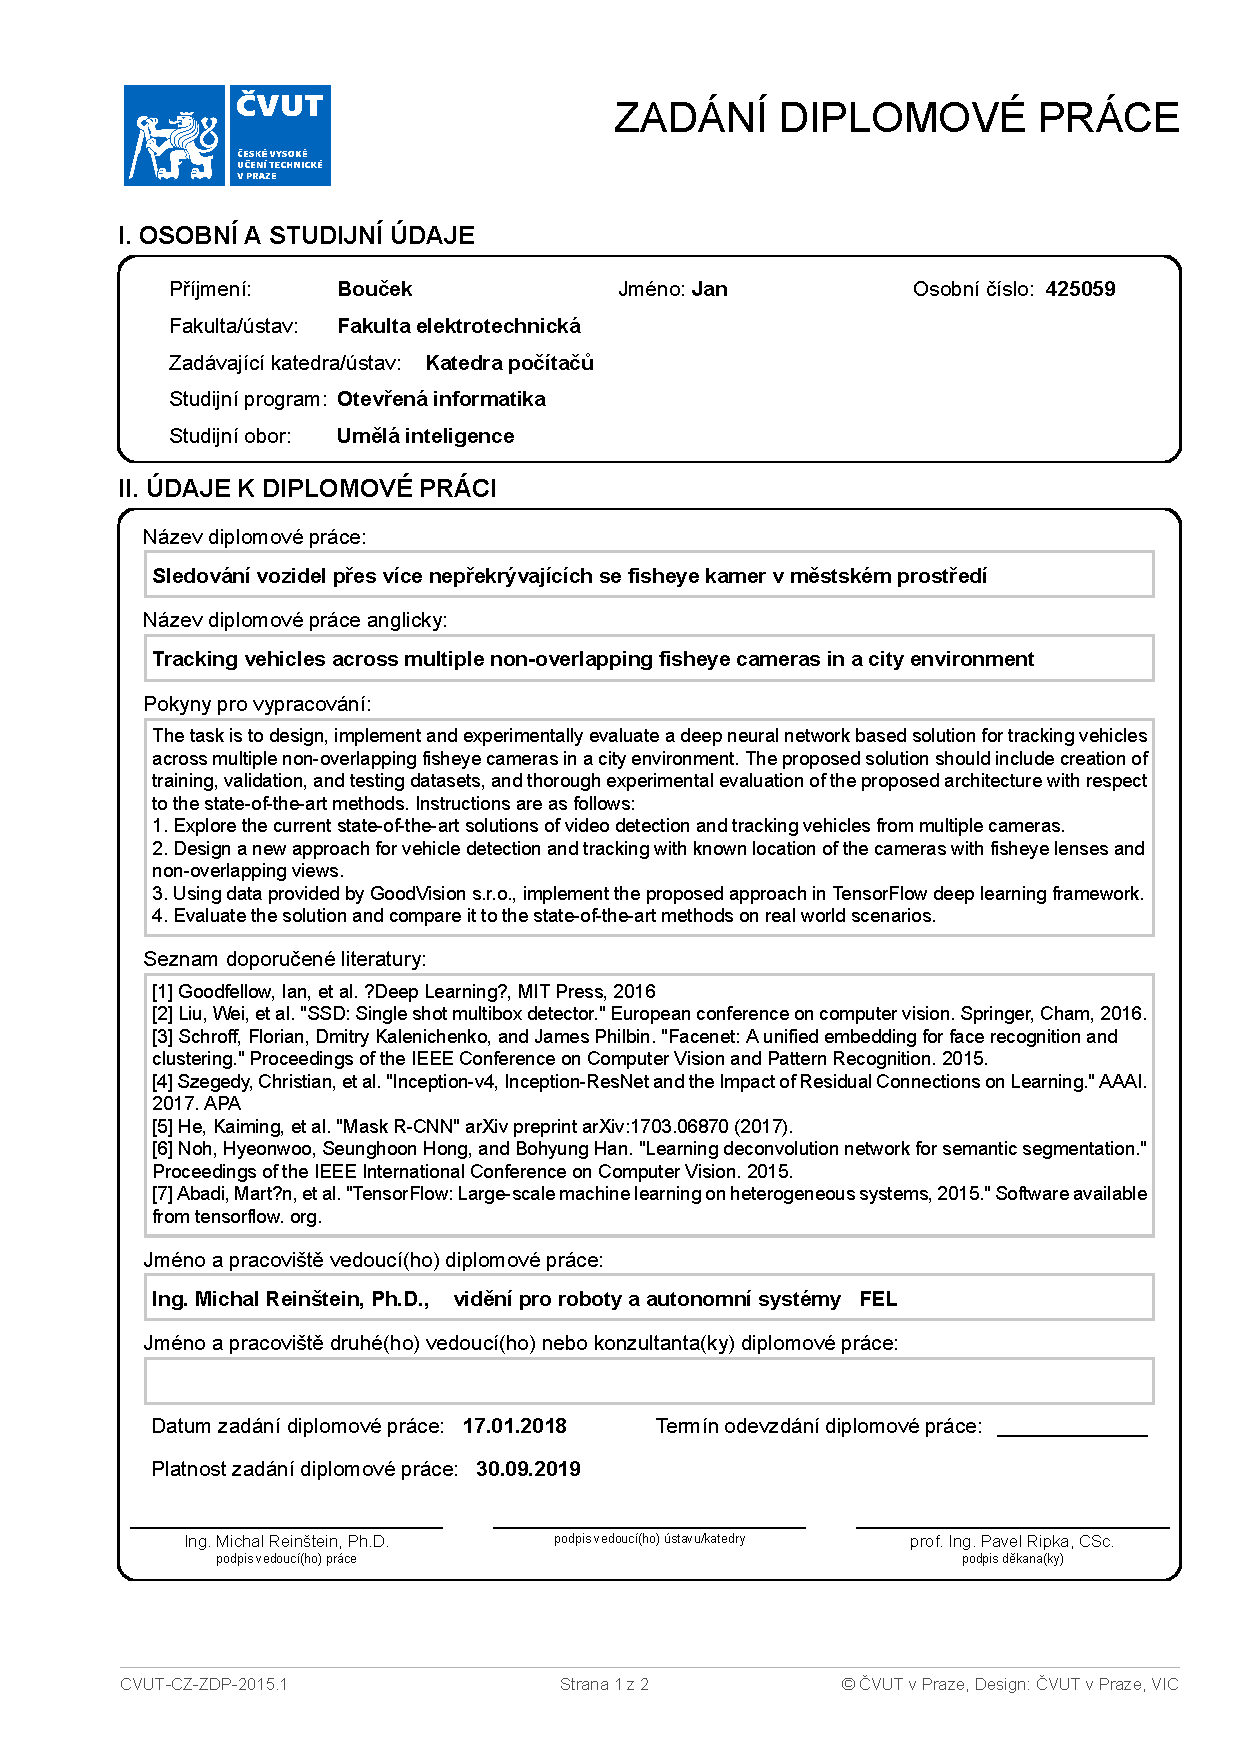
\includepdf[pages={1}]{zadani.pdf}
\cleardoublepage
%%





% Podekování
~\vfill{}

\section*{Acknowledgements}
I would like to thank my thesis supervisor Ing. Michal Reinštein Ph.D for his great support, leadership and expertise that helped greatly during this thesis. I would also like to thank the Good Vision company for great cooperation. Finally, I thank my friends and family for their support during my whole studies.
\vspace{2.5cm}

\newpage{}

\cleardoublepage

% Stránka s abstrakty
\vfill
\begin{center}
{\it \large Abstract}
\vspace{0.2cm}

\begin{minipage}{0.8\textwidth}{

This thesis deals with tracking vehicles over multiple non-overlapping cameras. The goal is to design and implement a system able to detect vehicles in a city environment and track their position. The cameras have a fish-eye view and are mounted to street lamps. We present a deep neural network for vehicle detection utilizing the video information, a single camera vehicle tracking algorithm based on optical flow, a deep neural network trained to compute similarities between vehicles and a probabilistic graph representation of a city. The conducted real world experiments verified the capability of the whole system.
\\
\\
\textbf{Keywords}: Object detection, Multi camera tracking, fisheye cameras.
}
\end{minipage}
\end{center}
\vfill
\vspace{1cm}

\vfill
\begin{center}
{\it \large Abstrakt}
\vspace{0.2cm}

\begin{minipage}{0.8\textwidth}{
Tato práce se zabývá sledováním vozidel přes více nepřekrývajících se kamer. Cílem této práce je návrh a realizace systému, který je schopný rozpoznat vozidla v městském prostředí a sledovat jejich polohu. Kamery mají objektiv typu rybí oko a jsou umístěny do pouličních lamp. Představujeme hlubokou neuronovou síť pro detekci vozidel využívající informace z videa, algoritmus pro sledování vozidel na jedné kameře založený na optical flow, hlubokou neuronovou síť pro počítání podobností mezi vozidly a pravděpodobnostní grafovou reprezentaci města. Provedené experimenty reálného světa ověřily schopnosti celého systému.
\\
\\
\textbf{Klíčová slova}: Detekce objektů, sledování přes více kamer, objektiv rybí oko
}
\end{minipage}
\end{center}
\vfill
\vspace{1cm}
\newpage{}
\cleardoublepage

\pagestyle{fancy}
\pagenumbering{roman}
\cfoot{\thepage}

% Obsah
\tableofcontents
\cleardoublepage

% Seznam obrázků
\listoffigures
\cleardoublepage

\pagestyle{fancy}
\pagenumbering{arabic}
\cfoot{}
\rfoot{\thepage$/$\pageref{LastPage}}
\setlength{\parskip}{0.35cm}

\lhead{\emph{\leftmark}}
\rhead{}

% Úvod
\pdfoutput=1
\documentclass[a4paper,12pt,titlepage, twoside]{article}
\usepackage[english]{babel}
\usepackage[utf8]{inputenc}
\usepackage{amssymb,amsmath}
\usepackage{algorithm,algpseudocode}
\usepackage[title,titletoc]{appendix}

\begin{document}


\section{Introduction}

Computer vision field has incredibly improved over last 5 years. This has been mainly thanks to the convoluional neural networks, which can be used for a wide variety of tasks. Their rise has been made possible by incresing computational power and using GPUs. Accecibility of huge datasets, such as ImageNet\cite{imagenet}, Pascal VOC \cite{pascal} are also very important for training. 


\section{State of the Art}
The task of image recognition has been quite solved, . The Inception network \cite{inception}



\bibliographystyle{plain}
\bibliography{ref}{}
\cleardoublepage
\clearpage

\end{document}
\clearpage

% State of the art
% \input{src/related_work}	// muj comment
% \clearpage


\input{src/dynamics}
\clearpage

\input{src/mpc_formulation}
\clearpage


\input{src/mpc_implementation}
\clearpage

\input{src/avoidance}
\clearpage

\input{src/solving_lcqp}
\clearpage

\input{src/move_blocking}
\clearpage

\input{src/simulations}
\clearpage

\input{src/hardware}
\clearpage

\input{src/experiments}
\clearpage

% Závěr
\input{src/conclusion}
\cleardoublepage

% Seznam literatury se nachází v bp.bib
\bibliographystyle{plain}
\bibliography{bp}{}
\cleardoublepage
\clearpage


% Apendixy, schemata, seznam zkratek, atp...
\appendices
\lhead{\emph{APPENDIX \leftmark}} 
\section{CD Content}

In Table~\ref{tab:obsah} are listed names of directories on CD.

\vspace{1cm}
\begin{table}[!htb]
\centering
\begin{tabular}{lp{10cm}}
\hline
\textbf{Directory name} & \textbf{Description} \\
\hline
thesis & Bachelor's thesis in pdf format\\
STM & sources for STM32F4 \\
xMega & sources for ATxMega128A3U \\
Matlab & matlab scripts for simulation \\
videos & videos from experiments \\
\hline
\end{tabular}
\caption{CD Content}
\label{tab:obsah}
\end{table}.
\clearpage

\section{List of abbreviations}\label{ape:abbreviations}

In Table \ref{table:abbreviations} are listed abbreviations used in this thesis.

\begin{table}[!htb]
\centering
\begin{tabular}{ll}
\hline
\textbf{Abbreviation} & \textbf{Meaning} \\
\hline

\textbf{CPU} & control processing unit \\
\textbf{GPU} & graphic processing unit \\
\textbf{VOC} & The PASCAL Visual Object Classes\\
\textbf{SVM} & support vector machine \\
\textbf{SSD} & Single Shot MultiBox Detector \\
\textbf{YOLO} & you only look once \\

\hline
\end{tabular}
\caption{Lists of abbreviations}
\label{table:abbreviations}
\end{table}

\end{document}
